\documentclass{article}
\usepackage{graphicx} % Required for inserting images
\usepackage{color}
\usepackage{listings}
\usepackage{courier}
\usepackage{tabularx}

\lstloadlanguages{% Check Dokumentation for further languages ...
%[Visual]Basic
%Pascal
C,
C++,
csh,
%XML
%HTML
Java
}
\definecolor{red}{rgb}{0.6,0,0} % for strings
\definecolor{blue}{rgb}{0,0,0.6}
\definecolor{green}{rgb}{0,0.8,0}
\definecolor{cyan}{rgb}{0.0,0.6,0.6}

\lstset{
language=csh,
basicstyle=\footnotesize\ttfamily, % Standardschrift
numbers=left, % Ort der Zeilennummern
numberstyle=\tiny, % Stil der Zeilennummern
%stepnumber=2, % Abstand zwischen den Zeilennummern
numbersep=5pt, % Abstand der Nummern zum Text
tabsize=2, % Groesse von Tabs
extendedchars=true, %
breaklines=true, % Zeilen werden Umgebrochen
%keywordstyle=\color{red}\bfseries,
frame=b,
%keywordstyle=[1]\textbf, % Stil der Keywords
% keywordstyle=[2]\textbf, %
% keywordstyle=[3]\textbf, %
% keywordstyle=[4]\textbf, \sqrt{\sqrt{}} %
stringstyle=\color{blue}\ttfamily, % Farbe der String
showspaces=false, % Leerzeichen anzeigen ?
showtabs=true, % Tabs anzeigen ?
xleftmargin=17pt,
framexleftmargin=17pt,
framexrightmargin=5pt,
framexbottommargin=4pt,
commentstyle=\color{blue},
morecomment=[s][\color{green}]{//}{},
%backgroundcolor=\color{grey},
showstringspaces=false, % Leerzeichen in Strings anzeigen ?
%morekeywords={__global__} % CUDA specific keywords
morekeywords={  abstract, event, new, struct,
                as, explicit, null, switch,
                base, extern, object, this,
                bool, false, operator, throw,
                break, finally, out, true,
                byte, fixed, override, try,
                case, float, params, typeof,
                catch, for, private, uint,
                char, foreach, protected, ulong,
                checked, goto, public, unchecked,
                class, if, readonly, unsafe,
                const, implicit, ref, ushort,
                continue, in, return, using,
                decimal, int, sbyte, virtual,
                default, interface, sealed, volatile,
                delegate, internal, short, void,
                do, is, sizeof, while,
                double, lock, stackalloc,
                else, long, static,
                enum, namespace, string},% list your attributes here
keywordstyle=\color{cyan},
identifierstyle=\color{red},
}
%\DeclareCaptionFont{blue}{\color{blue}}

%\captionsetup[lstlisting]{singlelinecheck=false, labelfont={blue}, textfont={blue}}
\usepackage{caption}
\DeclareCaptionFont{white}{\color{white}}
\DeclareCaptionFormat{listing}{\colorbox{8}{\parbox{\textwidth}{\hspace{15pt}#1#2#3}}}
\captionsetup[lstlisting]{format=listing,labelfont=white,textfont=white, singlelinecheck=false, margin=0pt, font={bf,footnotesize}}

\lstset{       % keyword style
  language=csh,
  }



\usepackage{graphicx} % Required for inserting images
\usepackage{listings}
\usepackage{color}
\usepackage{hyperref}
\lstloadlanguages{C,C++,csh,Java}
\usepackage{pdfpages}

\begin{document}


\includepdf[pages = 1, fitpaper]{coverpage}

\titlepage 
\tableofcontents
\newpage
\thispagestyle{empty}
\listoffigures
\newpage
\thispagestyle{empty}
\listoftables
\newpage
\lstlistoflistings
\newpage
\pagenumbering{arabic}

\pagebreak
\section*{\huge Section 1}
\section{Introduction}

The modern definition of information security involves the protection of information assets, and components that facilitate the storage, usage, and transmission of the said information – emphasis being on the protection of information to preserve its confidentiality, integrity, and availability (Singh, 2003).
According to Pfleeger \emph{et al.,} (2015:74), encryption is the process of encoding a message so that its contents are concealed, and decryption is the reverse of such a process – the decoding of the message to understand its’ meaning. 

This project evaluates 4 types of cryptography methods (Vigenère, Transposition, Vernam, and Custom ciphers) and how each method is implemented to achieve encryption of the messages and files.

\subsection{Vigenère Cipher}
The Vigenère cipher, the first of its kind since the invention of the Caesar cipher, was created in the middle of the sixteenth century. It was created by Blaise de Vigenère, a former diplomat turned scholar, and published in 1856.
 
\subsubsection{Implementation of the Vigenère Cipher}
The Vigenère uses a simple polyalphabetic substitution method, where the plaintext is encrypted using a unique key, and the letters are shifted in terms of the key.
  
\paragraph{Messages\\}

\textbf{Encryption} 
Takes in two parameters, plaintext, and key, and returns a cipher text. Then uses a Dictionary to store all of the alphabet indexes from A to Z, A being 0 and Z being 25. If the character is not a letter, the algorithm appends the cipher text as it is. If the character is a letter, the algorithm calculates the index of the letter in plaintext and the cipher key using the ’AlphabetOrder Dictionary’, which arranges the letters in alphabetical order based on their position. It uses the FirstOrDefault method, which obtains the first element of the resulting sequence, or the default value if no element is found. The algorithm calculates the sum of two indexes obtained from the plaintext and the cipher key and then takes the modulus of 26. This index is then used to retrieve the corresponding letter from the Alphabet Order dictionary. The final index of the plaintext is retrieved in alphabetical order. The processed characters in the plaintext are then used to generate the ciphertext.\\

\textbf{Decryption}
The decryption process follows the same steps as the encryption process, with one exception. Instead of calculating the sum of two indexes obtained from the plaintext and the cipher key, the algorithm calculates their difference. The modulus of 26 is then applied to ensure that the resulting index is within the valid range and returns the plaintext.

\begin{lstlisting}[caption=Vigenère Cipher Text Source Code]
    class VigenereText
    {
        public String VigenereTextEncrypt(String plain, String cipherKey)
        {
            Dictionary<sbyte, char> AlphabetOrder = new Dictionary <sbyte, char> ();

            AlphabetOrder.Add(0, 'A'); 
            .........................
            AlphabetOrder.Add(25, 'Z');

            cipherKey = cipherKey.ToUpper();
            plain = plain.ToUpper();

            int i = 0;
            string encryptedText = "";


            try {
                foreach (char elements in plain)
                {
                    if (!Char.IsLetter(elements))
                    {
                        encryptedText += elements;
                    }
                    else
                    {
                        sbyte firstOrder = AlphabetOrder.FirstOrDefault(j => j.Value == elements).Key; 
                        sbyte lastOrder = AlphabetOrder.FirstOrDefault(j => j.Value == cipherKey[i]).Key;
                        sbyte finalValue = (sbyte)(firstOrder + lastOrder); 
                        
                        if (finalValue > 25) 
                        {
                            finalValue -= 26;
                        }
                        encryptedText += AlphabetOrder[finalValue]; 
                        i++;
                    }
                    if (i == cipherKey.Length) 
                    {
                        i = 0;
                    }
                }
                return encryptedText;
            } catch 
            {
                MessageBox.Show("Error", "Error", MessageBoxButtons.OK, MessageBoxIcon.Error);
            }
        }

        public String VigenereTextDecrypt(String mixed, String cipherKey)
        {
            Dictionary <sbyte, char> AlphabetOrder = new Dictionary <sbyte, char>();

            AlphabetOrder.Add(0, 'A'); 
            .........................
            AlphabetOrder.Add(25, 'Z');

            cipherKey = cipherKey.ToUpper();
            mixed = mixed.ToUpper();
            string decryptedText = "";

            int i = 0;

            try
            {
                foreach (char elements in mixed)
                {
                    if (!Char.IsLetter(elements))
                    {
                        decryptedText += elements;
                    }
                    else
                    {
                        sbyte firstOrder = AlphabetOrder.FirstOrDefault(j =>j.Value == elements).Key; 
                        sbyte lastOrder = AlphabetOrder.FirstOrDefault(j => j.Value == cipherKey[i]).Key;
                        sbyte finalValue = (sbyte)(firstOrder - lastOrder);
                        if (finalValue < 0) 
                        {
                            finalValue += 26;
                        }
                        decryptedText += AlphabetOrder[finalValue]; 
                        i++;
                    }
                    if (i == cipherKey.Length) 
                    {
                        i = 0;
                    }
                }
                return decryptedText;
            }
            catch 
            {
                MessageBox.Show("Error", "Error", MessageBoxButtons.OK, MessageBoxIcon.Error);
            }
        }
    }
\end{lstlisting}

\paragraph{Files\\}
The Vigenère can encrypt files as strings or bytes, in this case bytes. In our implementation, the key is usually generated so that it can be used with ease in the decryption method. When it encrypts, it converts the contents into non-alphabetic ones. If it is a text file, it converts each character to the corresponding letter; A becomes 0, and so on. The extension of the file is usually changed to "vig" to show that it is encrypted, and it uses the same method to decrypt and uses the generated key.

\begin{lstlisting}[caption=Vigenère Cipher File Source Code]
public void VigenereFileDecrypt(string encryptedFiles, string keyFile, string decryptedFile)
{
    byte[] encryptedBytes;

    using (FileStream fileStream = new FileStream(encryptedFiles, FileMode.Open))
    {
        encryptedBytes = new byte[fileStream.Length];
        fileStream.Read(encryptedBytes, 0, encryptedBytes.Length);
    }

    byte[] bytesOfKey;
    using (FileStream fileStream = new FileStream(keyFile, FileMode.Open))
    {
        bytesOfKey = new byte[fileStream.Length];
        fileStream.Read(bytesOfKey, 0, bytesOfKey.Length);            
            
        byte[] decryptedData = new byte[encryptedBytes.Length];
        VigenereEncrypt(encryptedBytes, bytesOfKey, ref decryptedData);
        if (encryptedFiles.Contains(".vig"))
        {
            encryptedFiles.Replace(".vig", "");
            using (FileStream fileStream = new FileStream(decryptedFile, FileMode.Create))
            {
                fileStream.Write(decryptedData, 0, decryptedData.Length);
            }
        }
        else
        {
            using (FileStream fileStream = new FileStream(decryptedFile, FileMode.Create))
                {
                    fileStream.Write(decryptedData, 0, decryptedData.Length);
                }
        }
    }
}
\end{lstlisting}

\subsection{Transposition Cipher}
A transposition cipher is a type that scrambles the order of letters. One of the oldest ways to scramble words in this form was created in ancient Greece by the Egyptians and Greeks. 

\subsubsection{Implemetation of the Transposition Cipher}

\paragraph{Messages\\}

It uses an abstract class to implement security algorithms, including an alphabet dictionary, and has a constructor that initializes the object alphabet dictionary. The algorithm has two abstract classes, encrypt and decrypt, which are used in this project. The algorithm inherits from the CreateDictionary class, with a constructor that takes the key and determines the number of rows in the transposition matrix. 

It uses two major functions that will be discussed further which are called: 
\begin{itemize}
    \item The Transpose() method takes in two parameters. The value of the encryption key determines the number of rows and based on the length of the message and the key, it calculates the number of rows and columns in the transposition matrix. This method then calls a private method called FillArray, which creates a 2-dimensional char array representing the transposition matrix. 
    \item The FillArray() method fills the remaining positions with asterisks (*) if there are no characters left in the plain text to fill the positions in the columns.
\end{itemize}

\begin{lstlisting}[caption=Transposition Cipher Text Source Code]
class TranspositionText : CreateDictionary
    {
        private string TransposeText(string textMessage, Mode newMode) 
        {
            string finalText = "";
            int records = encryptionKey;
            int fields = (int)Math.Ceiling((double)textMessage.Length / (double records);
            char[,] matrixSize = FillArray(textMessage, records, fields, newMode);
            
            foreach (char c in matrixSize)
            {
                finalText += c;
            }
            return finalText;
        }

        private char[,] FillArray(string textMessage, int numberOfRows, int numberOfColumns, Mode newMode) 
        {
            int charPositionInArr = 0; 
            int lengthOfArr = 0, widthOfArr = 0; 
            char[,] matrixSize = new char[numberOfRows, numberOfRows]; 

            switch (newMode)
            {
                case Mode.Encrypt:
                    lengthOfArr = numberOfRows;
                    widthOfArr = numberOfRows;
                    break;
                case Mode.Decrypt: 
                    matrixSize = new char[numberOfRows, numberOfRows];
                    widthOfArr = numberOfRows;
                    lengthOfArr = numberOfRows;
                    break;
            }

            for (int i = 0; i < widthOfArr; i++)
            {
                for (int j = 0; j < lengthOfArr; j++)
                {
                    if (charPositionInArr < textMessage.Length)
                    {
                        matrixSize[j, i] = textMessage[charPositionInArr]; 
                    }
                    else
                    {
                        matrixSize[j, i] = '*'; 
                    }

                    charPositionInArr++;
                }
            }
            return matrixSize; 
        }
        internal enum Mode 
        {
            Encrypt, Decrypt
        }
    }
\end{lstlisting}

\paragraph{Files\\}
It uses the same key to encrypt and decrypt. It uses a method called Transpose that takes in three parameters, which include the input, output, and status of the encryption method. The status is the one that will be used in the buttons to determine whether it has to encrypt or decrypt . The transpose method is the one that converts the content of the file into bytes. A key is usually generated after encrypting the file, it can be used to decrypt the file.\\
\\
\\

\begin{lstlisting}[caption=Transposition Cipher File Source Code]
public void Transpose(string input, string output, int status)
        {
            byte[] bytes;

            using(FileStream fileStream = new FileStream(input, FileMode.Open))
            {
                bytes = new byte[fileStream.Length];
                fileStream.Read(bytes, 0, bytes.Length);    
            }

            byte[] inputArr = bytes;
            Array.Reverse(inputArr, 0, inputArr.Length);

            if (status == 1)
            {
                using(FileStream fileStream = new FileStream(output + ".trans", FileMode.Create)) {
                    fileStream.Write(inputArr, 0, inputArr.Length);
                }
            } else
            {
                if(input.Contains(".trans"))
                {
                    input.Replace(".trans", " ");
                    using (FileStream fileStream = new FileStream(output, FileMode.Create))
                    {
                        fileStream.Write(inputArr, 0, inputArr.Length);
                    } 
                } else
                {
                    using (FileStream fileStream = new FileStream(output,FileMode.Create))
                    {
                        fileStream.Write(inputArr, 0, inputArr.Length);
                    }
                }
            }

        }
\end{lstlisting}

\subsection{Vernam Cipher}
The Vernam cipher was invented by Gilbert Sandford Vernam (1890-1960) in 1918. The Vernam Cipher is based on randomization. The plaintext character from a message is mixed with one character stream from a key stream. If the keystream was indeed random, the resulting ciphertext will also be random with no relation to the plaintext. To create the ciphertext, the logical operator (exclusive-or) XOR is applied to the individual bits of the plaintext and the key stream.

\subsubsection{Implementation of the Vernam Cipher}

\paragraph{Messages\\}
The encryption algorithm uses XOR (exclusive OR) to encrypt and decrypt. It first stores the encrypted or decrypted text and iterates through the plain text. It uses the XOR operations in the plain text, the character, and the cipher text will be stored in a variable which will be the one that is encrypted.\\ 
\\It takes the remainder of the cipher text and calculates the index of the key character for the plain text and divides it by the length of the key which ensures that the key is used in both operations (encryption and decryption). The key character will be retrieved from the plaintext and the index of the key, and this key will be used in the XOR operation. The XOR operator then compares each bit of the two operands and produces a result.



\begin{lstlisting}[caption=Vernam Cipher Text Source Code]
namespace Cryptography_Project.Vernam
{
    internal class VernamText
    {
        public string VernamEncryptionAndDecryption(string plainText, string key)
        {
            var encryptedText = new StringBuilder(); 

            for (int cipherText = 0; cipherText < plainText.Length; cipherText++) 
            {
                char character = plainText[cipherText]; 

                uint charCode = (uint)character; 

                int keyPosition = cipherText % key.Length; 

                //take the key character at the calculated index
                char keyChar = key[keyPosition]; 

                uint keyCode = (uint)keyChar; 

                uint combinedCode = charCode ^ keyCode; 

                char combinedChar = (char)combinedCode; 

                encryptedText.Append(combinedChar);
            }
            return encryptedText.ToString();
        }
    }
}
\end{lstlisting}

\paragraph{Files\\}
\textbf{Encryption}
The Vernam algorithm takes in 3 parameters which are input, output, and key. There is an array of bytes that will be utilized to read the original file. The FileStream class is used to read the input file into the byte array. When it reads the file, it also generates a random key with the exact length of the original file, the key is containing random bytes. Then it writes the key bytes into the key. It creates a duplicate array of the original byte array and is passed to the encryption method. Then bytes are written into the file.\\

\textbf{Decryption}
It works the same way as the Encryption, just that when it decrypts it takes in the key that was generated by the encryption method to decrypt the file.\\

\textbf{Method}
The encryption method takes in three parameters, inputArray, keyArray, and outputArray. It checks whether all those parameters have the same length, then start with the XOR to create a new array.

\begin{lstlisting}[caption=Vernam Cipher File Source Code]
internal class VernamFiles
    {
        public void VernamFileEncrypt(string inputFile, string encryptedFile, string keyFile)
        {
            byte[] originalBytes; 

            byte[] keyBytes = new byte[originalBytes.Length];                      
            Random rand = new Random();                                            
            rand.NextBytes(keyBytes);                                               

            byte[] encryptedBytes = new byte[originalBytes.Length];                
            VernamEncrypt(originalBytes, keyBytes, ref encryptedBytes);            
        }

        private void VernamEncrypt(byte[] inputBytes, byte[] keyBytes, ref byte[] outBytes)
        {
            if (inputBytes.Length != keyBytes.Length || (keyBytes.Length != outBytes.Length))
            {
                MessageBox.Show("The length of the original, key, and cipher must be the same.", "Error", MessageBoxButtons.OK, MessageBoxIcon.Error);
            }
            else
            {
                for (int i = 0; i < inputBytes.Length; i++)
                {
                    outBytes[i] = (byte)(inputBytes[i] ^ keyBytes[i]);
                }
            }
        }

        public void VernamFileDecrypt(string encryptedFiles, string keyFile, string decryptedFile)
        {
            byte[] encryptedBytes;

            using (FileStream fileStream = new FileStream(encryptedFiles, FileMode.Open))
            {
                encryptedBytes = new byte[fileStream.Length];
                fileStream.Read(encryptedBytes, 0, encryptedBytes.Length);
            }

            byte[] keyFileBytes;
            using (FileStream fileStream = new FileStream(keyFile, FileMode.Open))
            {
                keyFileBytes = new byte[fileStream.Length];
                fileStream.Read(keyFileBytes, 0, keyFileBytes.Length);
            }

            byte[] decryptedData = new byte[encryptedBytes.Length];
            VernamEncrypt(encryptedBytes, keyFileBytes, ref decryptedData);

            if (encryptedFiles.Contains(".ver"))
            {
                encryptedFiles.Replace(".ver", "");
                using (FileStream fileStream = new FileStream(decryptedFile, FileMode.Create))
                {
                    fileStream.Write(decryptedData, 0, decryptedData.Length);
                }
            }
            else
            {
                using (FileStream fileStream = new FileStream(decryptedFile, FileMode.Create))
                {
                    fileStream.Write(decryptedData, 0, decryptedData.Length);
                }
            }
        }
    }
\end{lstlisting}
\subsection{B\&G InHouse}

Our in-house method, called B\&G InHouse, is a custom solution that we developed ourselves. The method employs an ASCII Table to create a custom cipher, which involves three steps: swapping characters, reversing them, and shifting them using the ASCII Table

\begin{table}[hbt!]
\begin{tabular}{|c|c|c|c|c|c|c|c|c|c|c|c|c|c|c|c|}
\hline
0  & \textbf{NUL} & 16 & \textbf{DLE} & 32 & \textbf{SP} & 48 & \textbf{0}              & 64 & \textbf{@} & 80 & \textbf{P}                  & 96  & \textbf{`} & 112 & \textbf{p}      \\ \hline
1  & \textbf{SOH} & 17 & \textbf{DC1} & 33 & \textbf{!}  & 49 & \textbf{1}              & 65 & \textbf{A} & 81 & \textbf{Q}                  & 97  & \textbf{a} & 113 & \textbf{q}      \\ \hline
2  & \textbf{STX} & 18 & \textbf{DC2} & 34 & \textbf{"}  & 50 & \textbf{2}              & 66 & \textbf{B} & 82 & \textbf{R}                  & 98  & \textbf{b} & 114 & \textbf{r}      \\ \hline
3  & \textbf{ETX} & 19 & \textbf{DC3} & 35 & \textbf{\#} & 51 & \textbf{3}              & 67 & \textbf{C} & 83 & \textbf{S}                  & 99  & \textbf{c} & 115 & \textbf{s}      \\ \hline
4  & \textbf{EOT} & 20 & \textbf{DC4} & 36 & \textbf{\$} & 52 & \textbf{4}              & 68 & \textbf{D} & 84 & \textbf{T}                  & 100 & \textbf{d} & 116 & \textbf{t}      \\ \hline
5  & \textbf{ENQ} & 21 & \textbf{NAK} & 37 & \textbf{\%} & 53 & \textbf{5}              & 69 & \textbf{E} & 85 & \textbf{U}                  & 101 & \textbf{e} & 117 & \textbf{u}      \\ \hline
6  & \textbf{ACK} & 22 & \textbf{SYN} & 38 & \textbf{\&} & 54 & \textbf{6}              & 70 & \textbf{F} & 86 & \textbf{V}                  & 102 & \textbf{f} & 118 & \textbf{w}      \\ \hline
7  & \textbf{BEL} & 23 & \textbf{ETB} & 39 & \textbf{'}  & 55 & \textbf{7}              & 71 & \textbf{G} & 87 & \textbf{W}                  & 103 & \textbf{g} & 119 & \textbf{v}      \\ \hline
8  & \textbf{BS}  & 24 & \textbf{CAN} & 40 & \textbf{(}  & 56 & \textbf{8}              & 72 & \textbf{H} & 88 & \textbf{X}                  & 104 & \textbf{h} & 120 & \textbf{z}      \\ \hline
9  & \textbf{HT}  & 25 & \textbf{EM}  & 41 & \textbf{)}  & 57 & \textbf{9}              & 73 & \textbf{I} & 89 & \textbf{Y}                  & 105 & \textbf{i} & 121 & \textbf{y}      \\ \hline
10 & \textbf{LF}  & 26 & \textbf{SUB} & 42 & *           & 58 & \textbf{:}              & 74 & \textbf{J} & 90 & \textbf{Z}                  & 106 & \textbf{j} & 122 & \textbf{z}      \\ \hline
11 & \textbf{VT}  & 27 & \textbf{ESC} & 43 & \textbf{+}  & 59 & \textbf{;}              & 75 & \textbf{K} & 91 & \textbf{{[}}                & 107 & \textbf{k} & 123 & \textbf{\{}     \\ \hline
12 & \textbf{FF}  & 28 & \textbf{FS}  & 44 & \textbf{,}  & 60 & \textbf{\textless{}}    & 76 & \textbf{L} & 92 & \textbf{\textbackslash{}}   & 108 & \textbf{l} & 124 & \textbf{|}      \\ \hline
13 & \textbf{CR}  & 29 & \textbf{GS}  & 45 & \textbf{-}  & 61 & \textbf{=}              & 77 & \textbf{M} & 93 & \textbf{{]}}                & 109 & \textbf{m} & 125 & \textbf{\}}     \\ \hline
14 & \textbf{SOH} & 30 & \textbf{RS}  & 46 & \textbf{.}  & 62 & \textbf{\textgreater{}} & 78 & \textbf{N} & 94 & \textbf{\textasciicircum{}} & 110 & \textbf{n} & 126 & \textbf{$\sim$} \\ \hline
15 & \textbf{SI}  & 31 & \textbf{US}  & 47 & \textbf{/}  & 63 & \textbf{?}              & 79 & \textbf{O} & 95 & \textbf{\_}                 & 111 & \textbf{o} & 127 & \textbf{DEL}    \\ \hline

\end{tabular}
\caption{ASCII Table}
\label{tab:table3}

\end{table}

\subsubsection{Implementation of the B\&G InHouse}
\paragraph{Messages\\}
Our custom code is very easy to implement but it is very hard to crack although it does not have any key. It uses two major functions which are swapping and reversing.

The swapping method takes in a string and swaps the first and the last letter of the string and takes out the middle letters of the string and inserts it back between the last and first letter to form a new string.

The second function which is the reverse text takes the whole message and uses a for loop to iterate through it and reverses the whole string and returns it. 
The custom algorithm implements both of these methods by taking in the plain text as an input and outputting the cipher text. It converts the input text into a character array and iterates each character in the array.

It performs an operation of moving each value character in the ASCII table forward by three positions, which is done by adding 3 when encrypting and removing three when decrypting.  The new string will be the encrypted text.

Example: it can encrypt "custom algorithm" to "hmynwtlqf\%rtyxzr”

\begin{itemize}
    \item Step 1: Swapping - custom algorithm = mustom algorithc
    \item Step 2: Reversing  - mustom algorithc = chtirogla mostum
    \item Step 3:ASCII Table - chtirogla mostum = hmynwtlqf\%rtyxzr\\
\end{itemize}


\begin{lstlisting}[caption=B\&G Cipher Text Source Code]
namespace Cryptography_Project.Custom
{
    internal class CustomText
    {
        public String swapText(String plainText)
        {
            int indexFirstPosition, indexLastPosition, temp;
            string newPlainText, middlePosition, firstPosition, lastPosition;

            indexFirstPosition = 0;                     //index of first position
            indexLastPosition = plainText.Length - 1;   //index of last position

            middlePosition = plainText.Substring(1, indexLastPosition - 1); //middle position

            //swapping the position of the first and last character
            temp = indexFirstPosition;                  
            indexFirstPosition = indexLastPosition;     
            indexLastPosition = temp;

            //getting the first and last character
            firstPosition = plainText.Substring(indexFirstPosition, 1); 
            lastPosition = plainText.Substring(indexLastPosition, 1);

            //new string
            newPlainText = firstPosition + middlePosition + lastPosition;

            return newPlainText;
        }

        public String reverseText(String inputText)
        {
            string reversedText = "";
            for (int i = inputText.Length - 1; i >= 0; i--) //for loop to reverse the string
            {
                reversedText += inputText[i];
            }
            return reversedText;
        }

        public String encryptedText(string plainText)
        {
            char[] charArray = plainText.ToCharArray();

            string newCipherText = "";
            char charInArray, newCharInArray;
            int ASCIIValue, newASCIIValue;

            for (int i = 0; i < plainText.Length; i++) //for loop to move each character 5 positions forward in ASCII table
            {
                charInArray = charArray[i];

                ASCIIValue = (char)charInArray;
                newASCIIValue = ASCIIValue + 5; //moving 5 positions forward in ASCII table

                newCharInArray = (char) newASCIIValue;
                newCipherText += newCharInArray;
            }
            return newCipherText;
        }

        public String decryptedText(string plainText)
        {
            char[] charArray = plainText.ToCharArray();

            string newCipherText = "";
            char charInArray, newCharInArray;
            int ASCIIValue, newASCIIValue;

            for (int i = 0; i < plainText.Length; i++)
            {
                charInArray = charArray[i];

                ASCIIValue = (char)charInArray;
                newASCIIValue = ASCIIValue - 5; //moving 5 positions backward in ASCII table

                newCharInArray = (char) newASCIIValue;
                newCipherText += newCharInArray;
            }
            return newCipherText;
        }
    }
}
\end{lstlisting}

\paragraph{Files\\}

This code uses a substitution cipher, which replaces one value with a different byte value based on the key generated from the password/key. 
It starts with a method called InitializeTable() for creating a substitution table for the substituting algorithm. The code initializes a byte array with byte values ranging from 0 to 255 and creates a two-dimensional byte array to hold the substitution table. The table array is then populated with unique byte values that are derived from the values in the first array, based on its position in the table. The generated substitution table will be used to encrypt and decrypt data using the substitution cipher algorithm

The file is read in as a byte array, and a key equal to the length of the file is created by duplicating the password up to that point. The algorithm then uses MD5 Cryptography and UTF8 Encoding to encrypt and decrypt data streams based on the ASCII values of the plaintext characters. The ASCII values of all characters in the input file are transformed and kept in a table array. The system gets a key from the user and converts it into bytes, which have the same length as the plaintext. 

A for loop is employed to shift the content of the original file by 256 values of a byte, and the plaintext is replaced with the corresponding ciphertext. Then, using an ASCII table it replaces each byte in the file with a different byte value based on the key. With the same file extension as the original file, the encrypted file is saved to the user's preferred location. To ensure that the encryption was effective, a message box finally appears.
To ensure security, the code uses a hashing algorithm called MD5 to convert the user's password into a fixed, shorter key value. This key is utilized to encrypt the file, and a matching MD5 hash of the password is required to decrypt it back to its original plaintext. Since the encryption and decryption use the same key, this is considered a symmetric cryptographic algorithm

This algorithm is effective since it uses MD5 with UTF8 encoding for authentication. 
\begin{itemize}
    \item MD5 is a cryptographic hash function and secure hash algorithm that can identify certain data corruption issues. It was primarily developed for the secure encryption of data during transmission and the authentication of digital certificates.
    \item UTF-8 is an encoding system designed for Unicode that enables the translation of any Unicode character to a unique binary string and vice versa.
\end{itemize}


\begin{lstlisting}[caption=B\&G Cipher File Source Code]
    public partial class CustomFileForm : Form
    {
        byte[] abcd;
        byte[,] byteTable;
        int k = 0;


        private void InitializeTable()
        {
            abcd = new byte[256];
            for (k = 0; k < 256; k++)
            {
                abcd[k] = Convert.ToByte(k);
            }

            byteTable = new byte[256, 256];
            for (int k = 0; k +< 256; k++)
            {
                for (int l = 0; l < 256; l++)
                {
                    byteTable[k, l] = abcd[(k + l) % 256];
                }
            }
        }
        
        private void Textbtn_Click(object sender, EventArgs e)
        {
                byte[] fileContents = File.ReadAllBytes(plainTextbox.Text);
                byte[] passwordTemp = Encoding.ASCII.GetBytes(passwordTextbox.Text);
                byte[] encryptionKey = new byte[fileContents.Length];
                byte[] encrypted = new byte[fileContents.Length];

                for (int k = 0; k < fileContents.Length; k++)
                {
                    encryptionKey[k] = passwordTemp[k % passwordTemp.Length];
                }
                
                if (encryptRadiobtn.Checked)
                {
                    for (int k = 0; k < fileContents.Length; k++)
                    {
                        byte valueofFile = fileContents[k];
                        byte cipherKey = encryptionKey[k];
                        int valueIndexes = -1, keyIndexes = -1;

                        for (int l = 0; l < 256; l++)
                        {
                            if (abcd[l] == valueofFile)
                            {
                                valueIndexes = l;
                                break;
                            }
                        }
                        for (int l = 0; l < 256; l++)
                        {
                            if (abcd[l] == cipherKey)
                            {
                                keyIndexes = l;
                            }
                        }
                        encrypted[k] = byteTable[keyIndexes, valueIndexes];
                    }
                }

                if (decryptRadiobtn.Checked)
                {
                    for (int k = 0; k < fileContents.Length; k++)
                    {
                        byte valueofFile = fileContents[k];
                        byte cipherKey = encryptionKey[k];
                        int valueIndexes = -1, keyIndexes = -1;

                        for (int l = 0; l < 256; l++)
                        {
                            if (abcd[l] == cipherKey)
                            {
                                keyIndexes = l;
                            }
                        }
                        for (int l = 0; l < 256; l++)
                        {
                            if (byteTable[keyIndexes, l] == valueofFile)
                            {
                                valueIndexes = l;
                                break;
                            }
                        }
                        encrypted[k] = abcd[valueIndexes];
                    }
                }
            }
        }
\end{lstlisting}

\newpage 
\section*{\huge Section 2}
\section{User Manual}
The application can be obtained either  a USB or by downloading it from GitHub.
\footnote{{\url:https://visualstudio.microsoft.com/vs//}}
The application can run on any Windows laptop it does not need any requirements. When the application is obtained, the user can click the setup.exe file and set up the application and follow the instructions below.

\subsection{Start Up}

When launching the application, you will be directed to the Start-Up page, which features a numbered layout of its components in the figure below, accompanied by a brief description for each corresponding number:

\begin{figure}[h!]
\centering
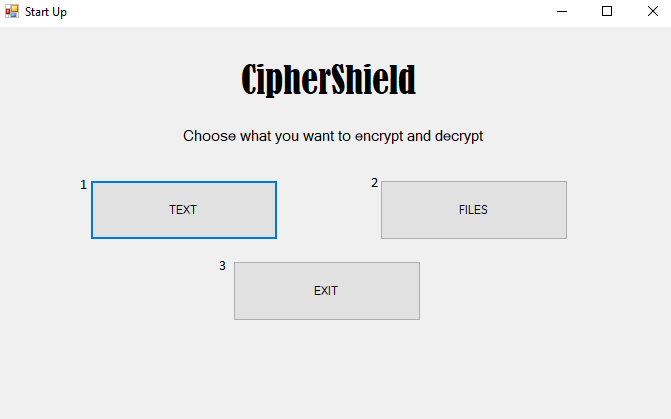
\includegraphics[scale=0.5]{Diagrams/StartU.png}
\caption{Start Up Page}
\label{fig:figure1}
\end{figure}

\begin{enumerate}
   \item This button will let you go to the Text Encryption Algorithms where you will encrypt and decrypt text.
   \item This button will direct you to the file encryption and decryption operations.
   \item Once you have finished using the application, simply click on this button to exit.
\end{enumerate}


\subsection{Text Encryption}
After clicking the Text you will be redirected to this Text Page which also has its own components:
\begin{figure}[h!]
\centering
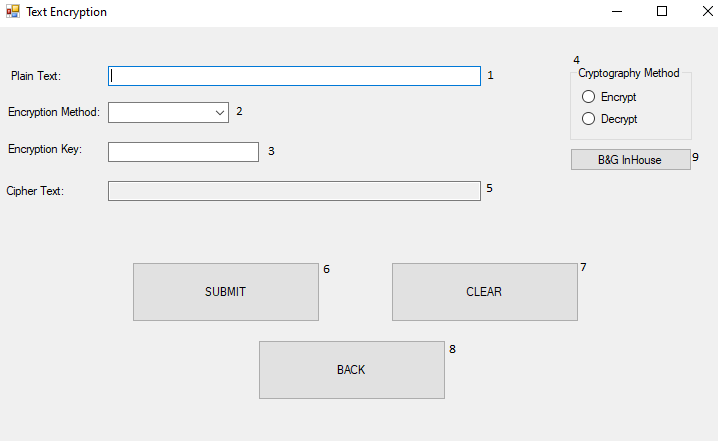
\includegraphics[scale=0.5]{Diagrams/TextEncryption.png}
\caption{Text Encryption Page}
\label{fig:figure1}
\end{figure}


\begin{enumerate}
   \item Textbox where you input the text you want to encrypt.
   \item Drop-down list for the different kinds of algorithms.
   \item Enter the key (note: keys differ with each algorithm).
   \item Radio buttons for encrypting or decrypting.
   \item After choosing numbers 1 - 4, press the submit button
   \item Output of the encrypted text.
   \item Clearing button to clear the textboxes, dropdown, and radio buttons.
   \item Back button to go back to the Start Up page.
   \item Going to the InHouse algorithm since it uses different operations than the other algorithms.
\end{enumerate}

\textbf{\\Instructions\\}
With regards to the text encryption methods: the user can input any message they want to encrypt and any key. \textbf{The Transposition and Vernam ciphers} only takes numbers as keys, and The \textbf{Vigenère cipher} takes letters only as encryption key. After putting in the key, you can choose any encryption method and choose to encrypt. When you want to decrypt make sure that the key is the same, if not it will not decrypt.

\subsubsection{B\&G InHouse}

After clicking the B\&G InHouse you will be redirected to this page which also has its own components:
\begin{figure}[h!]
\centering
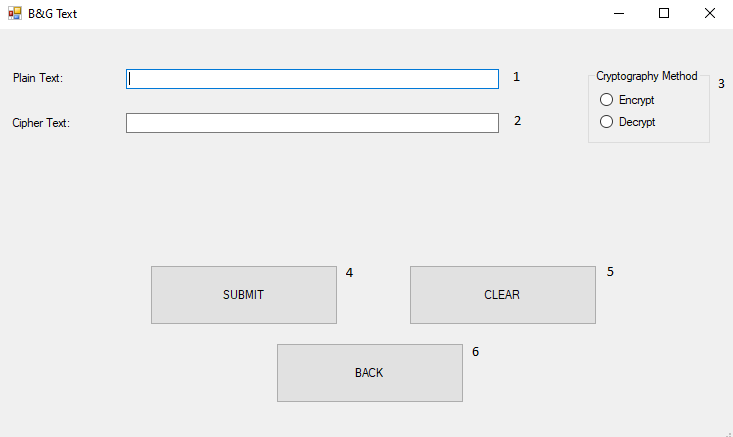
\includegraphics[scale=0.5]{Diagrams/custom.png}
\caption{B\&G Text Encryption Page}
\label{fig:figure1}
\end{figure}

\begin{enumerate}
   \item Textbox where you input the text you want to encrypt.
   \item Output of the encrypted text.
   \item Radio buttons for encrypting or decrypting.
   \item After choosing numbers 1 - 3, press the submit button
   \item Clearing button to clear the textboxes and radio buttons.
   \item Back button to go back to the Text Encryption page.

\end{enumerate}

\textbf{\\Instructions\\}
With B\&G InHouse, the user can simply enter the message they want to encrypt and choose a method. No key is needed.

\subsection{File Encryption}
After clicking the File button you will be redirected to this Text Page which also has its own components:

\begin{figure}[h!]
\centering
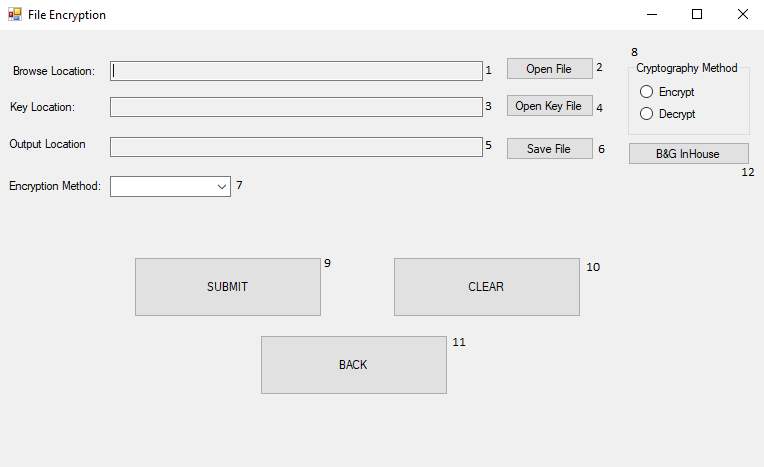
\includegraphics[scale=0.5]{Diagrams/FileEncryption.png}
\caption{File Encryption Page}
\label{fig:figure1}
\end{figure}

\begin{enumerate}
   \item Path of the file
   \item Button to locate the file you want to encrypt or decrypt.
   \item Path of the key file
   \item Button to locate the key file 
   \item Path of the output file
   \item Button to save the file 
   \item Drop-down list for the different encryption methods
   \item Radio buttons for encrypting or decrypting.
    \item After you are done, press the submit button
   \item Clearing button to clear the textboxes and radio buttons.
   \item Back button to go back to the File Encryption page.
   \item Button to go to the B\&G InHouse File Encryption.
\end{enumerate}

\textbf{\\Instructions\\}
With regards to the file encryption methods: the user can press the open file and choose any file they want to encrypt, the path of the file will be displayed, and the user will then choose a key file and  save the file that they want to encrypt. After that, they can choose any algorithm they want to use and choose to encrypt. When it is done a message will pop up. When you want to decrypt you select the decrypted file, in \textbf{Vernam cipher} you will select the key that is outputted and save the file, and press decrypt to get it to the original state. As well as the other algorithms.


\subsubsection{B\&G InHouse}
After clicking the B\&G InHouse you will be redirected to this page which also has its own components that will be discussed shortly.

To encrypt a file, you first select any file on your machine (such as docx, pdf, png, jpg, or any other file type), which will be displayed in the file path. Next, you enter a random key and choose to encrypt the file. Once you're done, press Submit and save the new file with any name you want. To decrypt the file, you follow the same steps but select the encrypted file instead.

\begin{enumerate}
   \item Path of the file
   \item Button to locate the file you want to encrypt or decrypt.
   \item The user does not need to input any key
   \item The user will generate any random key, the key for encrypting should be the same for encrypting
   \item Radio buttons for encrypting or decrypting.
   \item After you are done, press the submit button
   \item Clearing button to clear the textboxes and radio buttons.
   \item Back button to go back to the File Encryption page.
\end{enumerate}


\begin{figure}[h!]
\centering
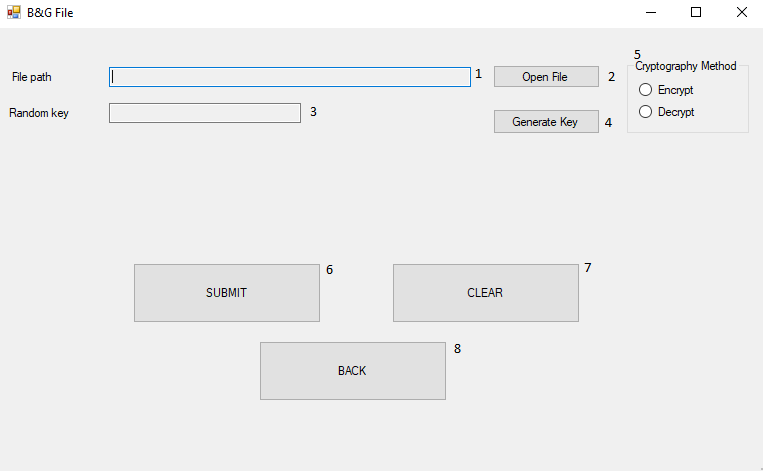
\includegraphics[scale=0.5]{Diagrams/customfil.png}
\caption{B\&G File Encryption Page}
\label{fig:figure1}
\end{figure}

\textbf{\\Instructions\\}
When you click Open File, you will go to any directory in your local machine, you select any file and click Open. The directory of the file will be shown in your File path on the application. Then you generate a random key, that will be used to encrypt and decrypt. It is a symmetrical key. You then click the Encrypt radio button and then Submit. It will lead you to the local directory where you have to name the new file. After naming it you will press save and the file will be encrypted. With encryption, you follow the same steps but you select the encrypted file and you select the decrypt radio button.
\\

\section*{\huge Section 3}

\section{Platforms Used}

In the development of our project, we have chosen to utilize both Visual Studio 2022 \footnote{{\url:https://visualstudio.microsoft.com/vs//}} and GitHub. \footnote{{\url{https://github.com/givenmnisi6/Cryptography-Project}}}

\subsection{Visual Studio 2022} 
For building, editing, and GUI (Graphical User Interfaces), as well as deploying applications, Visual Studio is the ideal platform to use. We utilized the .NET Framework in C\# to develop our application. We used it because of the following reasons (Microsoft, 2023): 

\begin{enumerate}
   \item Cross-platform compatibility: C\# is easy to develop applications in all Operating systems. Which makes it more versatile.
   \item Object-oriented programming: C\# is well suited for creating complex applications which support inheritance, abstract classes, and more
   \item Large community: In C\# there are a lot of resources that can assist you with troubleshooting.
\end{enumerate}

\subsection{GitHub}
In our project, we utilized GitHub throughout every development process. It makes version control easy and collaborates with others easily. We used it because of the following reasons (Kharlantseva, 2023): 


\begin{enumerate}
   \item Version control: makes it easy to track every process and allows for easy rollback to a stable version when changes have been made that break the code
   \item Integration with other apps: GitHub can easily integrate with other IDEs such as Visual Studio 2022 and many more. Making it easy to automate the development process

\end{enumerate}



\newpage
\section{Bibliography\\}

Kharlantseva, M. 2023, \emph{What Is GitHub? Everything You Need to Know} [Blog post]. \\
\url{https://everhour.com/blog/what-is-github/} Date of access: 16 May 2023. \\

Microsoft. 2023. \emph{Visual Studio Subscriptions and Benefits}.\\ \url{https://visualstudio.microsoft.com/subscriptions/} Date of access: 16 May 2023.\\

Pfleeger, C.P., Pfleeger, S.L. \& Margulies, J. 2015. \emph{Security in Computing (5th Edition)}. Prentice Hall Press.\\

Singh, S. 2003. The History of Cryptography: How the history of codebreaking can be used in the mathematics classroom with resources on a new CD-ROM. \emph{Mathematics in School}:2-6. 




\end{document}


\begin{document}

\maketitle
\input{Introduction}

\titlepage 
\tableofcontents


\end{document}

